\documentclass[14pt]{mmcs-article}
\usepackage[russian]{babel}
\usepackage{amsmath, amsthm, amsfonts, amssymb}

% После кванторов ставить отступ
% Починить \mod (\mathsc) -- сейчас там большой пробел в начале

% Надо бы настроить правильную сквозную нумерацию замечаний, теорем e.t.c

% Надо сделать примеры не в растре, а средствами теха

\graphicspath{{paper_images/}}

\begin{document}

\section*{Введение}

\textbf{Определение 1.}

% Надо потом аккуратно в замечении это всё дело переопределить так, чтобы запись была более компактная (отказаться от отображения, использовать пары)

\textsl{Двудольным графом} будем называть тройку $ G(V, E, f)$, такую, что:

\begin{itemize}
    \item $V = A \cup B$ и $A \cap B = \emptyset$ ;
    % Возможно надо использовать неупорядоченное декартово произведение, о том как это лучше сделать, надо смотреть в книжке Зыкова
    \item $f: E \rightarrow A \times B$ ;
\end{itemize}

Где $V$ ~-- множество вершин, разбитое на два непересекающихся подмножества $A$ и $B$.
$E$ ~-- множество дуг.
$f$ ~-- это отображение, определяющее то, с какими вершинами инцидентна дуга.

\textbf{Определение 2.}

Последовательность дуг $\mu = (e_1, ..., e_d)$ будем называть путём с начальной вершиной $v_0$ и конечной вершиной $v_d$  на графе $G(V,E,f)$, если существует последовательность вершин $(v_0, ..., v_d)$ такая, что $\forall i = 1,...,d:$ $(v_i, v_{i+1}) = f(e_i)$ или $(v_{i+1}, v_i) = f(e_i)$. 

% Пронумеровать вершины

Рассмотрим граф на рис \ref{image:1}. Последовательность дуг $(e_1, e_2, e_4, e_6)$ составляет путь с начальной вершиной C и конечной вершиной E.

\begin{figure}[H]
    \centering
    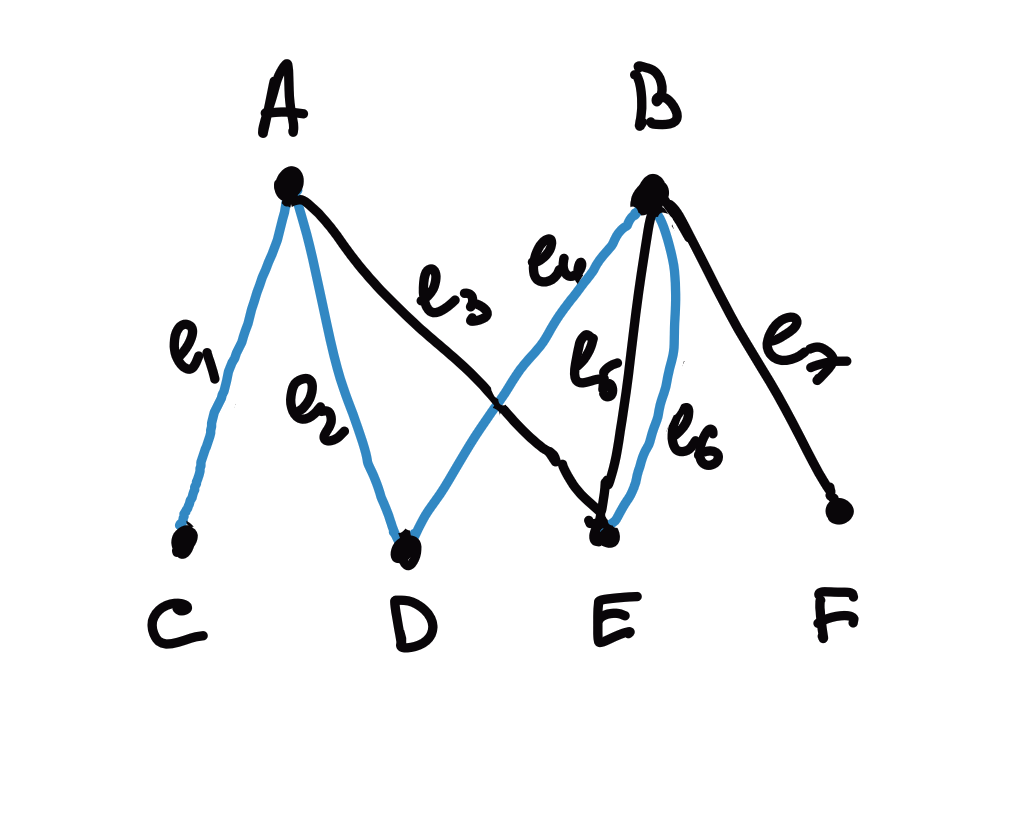
\includegraphics[scale=1.0]{path_example.png}
    \caption{ Двудольный граф. }\label{image:1}
\end{figure}

\textbf{Определение 4.}

\textsl{Циклом} будем называть путь, у которого совпадают первая и последняя вершины.

\textbf{Определение 6.}

\textsl{Обхватом графа} называют длину его минимального цикла.

\textbf{Замечание 1.}

Отметим, что обхват любого двудольного графа является чётным числом

% большим, чем два.

\textbf{Замечание 2.}

Известно, что на практике для кодирования эффективнее использовать графы с большим обхватом.

\textbf{Определение 5.}

% Характеристика дуги внутри пути (в какую сторону путь проходит дугу)

С каждым путём $\mu$ свяжем характеристическую функцию $\chi_\mu(e)$:
\[
    \begin{array}{ll}
        \chi_{\mu}(e_1) = \left\{
            \begin{array}{ll}
            1,  & v_0 \in A;\\
            -1, & v_0 \in B. \\
            \end{array}
        \right. \\
        \chi_\mu(e_i) = -\chi_\mu(e_{i-1}) \forall i \in 2, ..., d\\
    \end{array}
\]

\pagebreak
\section*{Метаграфы}

\textbf{Определение 6.}

Если $G(V,E,f)$ ~-- двудольный граф, то \textsl{Метаграфом} будем называть четвёрку $G'(V,E,f,w)$, где $w: E \to \mathbb{Z}$ ~-- отображения, задающее веса дуг

На рис. \ref{image:2} представлен метаграф  $G_1$ с тремя вершинами и четырьмя дугами.

\begin{figure}[H]
    \centering
    \begin{picture}(150,200)
        \put(75,165){\thicklines{\circle*{5}}}
        \put(70,170){$c_1$}
    
        \put(35,35){\thicklines{\circle*{5}}}
        \put(30,20){$i_1$}
    
        \put(115,35){\thicklines{\circle*{5}}}
        \put(110,20){$i_2$}
    
        \bezier{300}(75,165)(10,100)(35,35)
        \put(5,100){$+1$}

        \bezier{300}(75,165)(56,100)(35,35)
        \put(56,80){$0$}
    
        \bezier{300}(75,165)(140,100)(115,35)
        \put(125,100){$-1$}

        \bezier{300}(75,165)(94,100)(115,35)
        \put(87,80){$0$}
    \end{picture}
    \caption{ Метаграф с весами дуг +1, 0, 0, -1.. }
    \label{image:2}
\end{figure}

\textbf{Определение 7.}

Пусть $r \in \mathbb{N}$, тогда $r$-расширением метаграфа $G'(V,E,f,w)$ назовём граф $G^{(r)}(V^{(r)}, E^{(r)}, f^{(r)})$ построенный следующим образом:

\begin{itemize}
    \item Каждой вершине $v \in V$ соответствует множество вершин
    \[
        T^{(r)}(v) = \{ v^{(1)}, ..., v^{(r)} \}
    \]

    \item Тогда множество вершин метаграфа устроено следующим образом 
    \[
        V^{(r)} = \bigcup_{v \in V} T^{(r)}(v)
    \]

    \item Каждой дуге $e \in E$ соответствует множество дуг 
    \[
        T^{(r)}(e) = \{ e^{(1)}, ..., e^{(r)} \}
    \]

    \item Тогда множество дуг метаграфа устроено следующим образом
    \[
        E^{(r)} = \bigcup_{e \in E}T^{(r)}(e)
    \]

    \item Пусть $f(e) = (a, b)$, тогда $f^{(r)}(e^{(i)}) = (a^{(i)}, b^{(i + w(e) (\mod{r}))}) \forall i = 1,...,r$
\end{itemize}

На рис. \ref{image:3} изображён граф, полученный 4-расширением метаграфа $G_1$, изображённого на рис. \ref{image:2}.
% Пример нужен, чтобы показать, что на метаграфах с кратными дугами яразу появляются маленькие циклы

%% Забыл сделать дуги из первой в посленюю и обратно
\begin{figure}[H]
    \centering
    \begin{picture}(450,200)
        \put(75,165){\thicklines{\circle*{5}}}
        \put(70,170){$c_1$}
        \put(35,35){\thicklines{\circle*{5}}}
        \put(30,20){$i_1$}
        \put(115,35){\thicklines{\circle*{5}}}
        \put(110,20){$i_2$}

        \bezier{300}(75,165)(56,100)(35,35)
        \bezier{300}(75,165)(94,100)(115,35)
        \bezier{300}(75,165)(130,100)(135,35)
        \bezier{300}(175,165)(120,100)(115,35)

        \put(175,165){\thicklines{\circle*{5}}}
        \put(170,170){$c_1$}
        \put(135,35){\thicklines{\circle*{5}}}
        \put(130,20){$i_1$}
        \put(215,35){\thicklines{\circle*{5}}}
        \put(210,20){$i_2$}

        \bezier{300}(175,165)(156,100)(135,35)
        \bezier{300}(175,165)(194,100)(215,35)
        \bezier{300}(175,165)(230,100)(235,35)
        \bezier{300}(275,165)(220,100)(215,35)


        \put(275,165){\thicklines{\circle*{5}}}
        \put(270,170){$c_1$}
        \put(235,35){\thicklines{\circle*{5}}}
        \put(230,20){$i_1$}
        \put(315,35){\thicklines{\circle*{5}}}
        \put(310,20){$i_2$}

        \bezier{300}(275,165)(256,100)(235,35)
        \bezier{300}(275,165)(294,100)(315,35)
        \bezier{300}(275,165)(330,100)(335,35)
        \bezier{300}(375,165)(320,100)(315,35)


        \put(375,165){\thicklines{\circle*{5}}}
        \put(370,170){$c_1$}
        \put(335,35){\thicklines{\circle*{5}}}
        \put(330,20){$i_1$}
        \put(415,35){\thicklines{\circle*{5}}}
        \put(410,20){$i_2$}

        \bezier{300}(375,165)(356,100)(335,35)
        \bezier{300}(375,165)(394,100)(415,35)
    \end{picture}
    \caption{ Метаграф с весами дуг +1, 0, 0, -1.. }
    \label{image:3}
\end{figure}

\textbf{Теорема 1.} \textsl{(О начальных вершинах путей)}

Пусть $\eta = (e_1, \dots, e_d)$ ~-- путь с начальной вершиной $v$ на метаграфе $G$, тогда на графе $G^{(r)}$ существуют $r$ попарно не пересекающихся путей $\mu_1 \dots \mu_r$ с начальными вершинами $v^{(1)}, ..., v^{(r)}$, таких что для каждого пути $\mu'=(e_1',\dots,e_d') \in\{\mu_1,\dots,\mu_r\}$ справедливо, что для всех $j\in[1;d]_N$ $e_{j}' \in T^{(r)}(e_j)$.

\textbf{Доказательство.}

% Skorokhodov V.A. Generalization of the Reachability Problem on Directed Graphs/ Mathematics and Statistics, Vol. 8, No. 6, pp. 699 - 704, 2020. DOI: 10.13189/ms.2020.080610

Следует из определения расширения метаграфа.

\qed

\textbf{Определение 8.}

Будем говорить, что пути $\eta$ на метаграфе $G$ соответствуют пути $\mu_i$ на графе $G^{(r)}$ и наоборот.

\textbf{Замечание 2.}

Из того, что некоторый путь на метаграфе $G$ является циклом не следует, что соответствующие ему пути на $G^{(r)}$ являются циклами. Рассмотрим эту ситуацию на следующем примере.

\textbf{Пример 1.}

Рассмотрим граф на рис. \ref{image:4}. Путь $(e_1, e_2)$ является циклом на метаграфе, однако ни один из соответствующих ему путей $\mu_1 = (e^{(1)}_1, e^{(1)}_2)$, $\mu_2 = (e^{(2)}_1, e^{(2)}_2)$, $\mu_3 = (e^{(3)}_1, e^{(3)}_2)$  на 3-расширении не является циклом. При этом следует отметить, что склейка этих трёх путей порождает цикл $\mu = (e^{(1)}_1, e^{(1)}_2, e^{(2)}_1, e^{(2)}_2, e^{(3)}_1, e^{(3)}_2)$ длины 6. Заметим, что циклу $\mu$ соответствует цикл $(e_1, e_2, e_1, e_2, e_1, e_2)$ на метаграфе.

\begin{figure}[H]
    \centering
    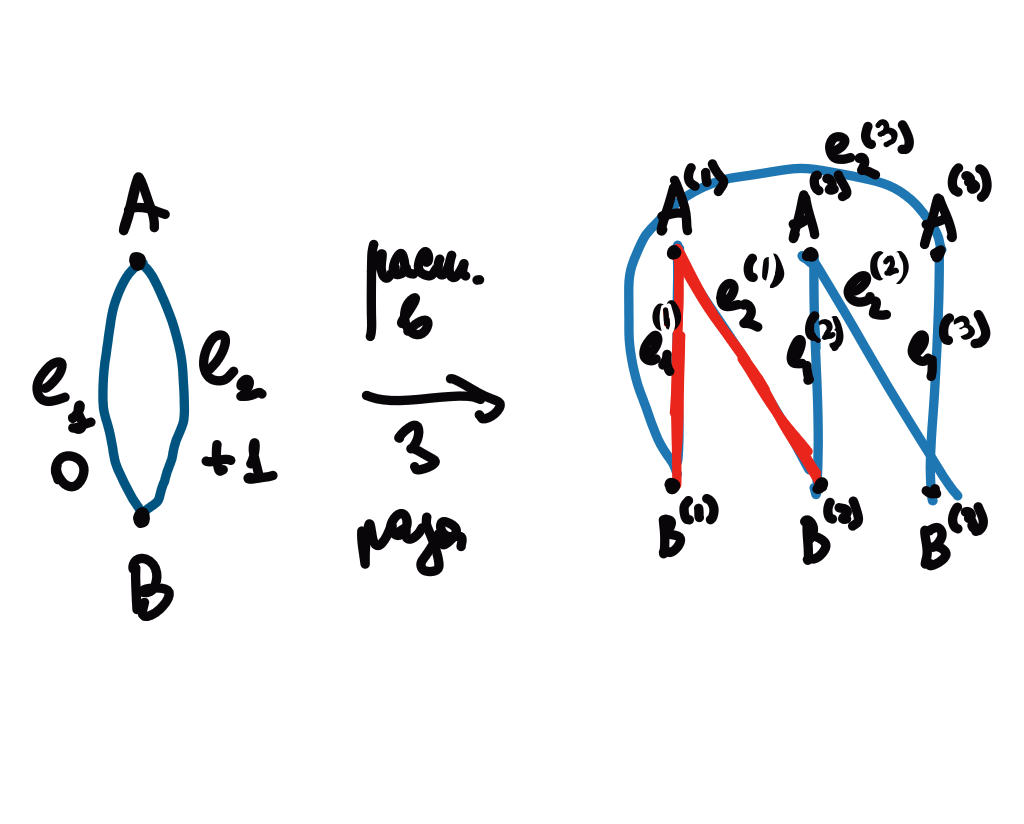
\includegraphics[scale=1.0]{cycle_on_metagraph_path_on_graph.png}
    \caption{ Путь соответствующий циклу $(e_1, e_2)$, не является циклом на графе-расширении. }\label{image:4}
\end{figure}


\textbf{Определение 7.}

Пусть $G(V, E, f, w)$ ~-- метаграф.

Характеристикой пути $\eta = (e_1, ..., e_d)$ будем называть

\[
    \chi(\eta) = \sum_{i = 1}^d \chi_{\eta}(e_i) w(e_i).
\]

\textbf{Теорема 2.}\textsl{(О конечных вершинах путей)}

Пусть  $\eta = (e_1, ..., e_d)$ ~-- путь на метаграфе $G$, его первая вершина ~-- $x$, а последняя вершина ~-- $y$. И пусть $\mu' = (e'_1, ..., e'_d)$ один из соответствующих ему путей на расширенном графе.

Тогда если у $\mu'$ начальная вершина $x^{(i)}$, то его последняя вершина ~-- $y^{(i + \chi(\eta)\mod{r})}$.

\textbf{Доказательство.}

% Как-то лучше мы это переписывали, а то просто месиво символов получается. Может там чуть ли не на "очевидно" можно было заменить

Доказательство проведём по индукции по длине пути $|\eta| = d$.

Пусть $d = 1$, тогда путь состоит их одной дуги $e_1$.

Если $x \in A$, тогда вершина $x^{(i)}$ инцидентна дуге $e_1'$, для которой $f^{(r)}(e_1') = (x^{(i)}, y^{(i + w(e_1) (\mod{r}))})$ то есть, конечной вершиной пути $\mu_i$ является $y^{(i + w(e_1) (\mod{r}))} = y^{(i + \chi(\eta) (\mod{r}))}$.

Если $x \in B$, тогда вершина $x^{(i)}$ инцидентна дуге $e_1'$, для которой $f^{(r)}(e_1') = (y^{(i - w(e_1) (\mod{r}))}, x^{(i)})$ то есть, конечной вершиной пути $\mu_i$ является $y^{(i - w(e_1) (\mod{r}))} = y^{(i + \chi(\eta) (\mod{r}))}$.

Пусть условия теоремы выполняются для всякого $d < n$, тогда рассмотрим случай $d = n$.

Рассмотрим путь $\eta' = (e_1, ..., e_{d - 1})$. Обозначим его последнюю вершину $x$. Тогда по предположению индукции последние вершины соответствующих ему путей на метаграфе ~-- это $x^{(i + \chi(\eta')(\mod{r}))}$.

Если $x \in A$, тогда вершина $x^{(i + \chi(\eta')(\mod{r}))}$ инцидентна дуге \\ $f^{(r)}(e_d^{(i + \chi(\eta')(\mod{r}))}) = (x^{(i + \chi(\eta')(\mod{r}))}, y^{(i + \chi(\eta') + w(e_d) (\mod{r}))})$ и конечная \\ вершина пути $\mu_i$ ~-- $y^{(i + \chi(\eta') + w(e_d) (\mod{r}))} = y^{(i + \chi(\mu) (\mod{r}))}$.

Если $x \in B$, тогда вершина $x^{(i + \chi(\eta')(\mod{r}))}$ инцидентна дуге \\ $f^{(r)}(e_d^{(i + \chi(\eta') - w(e_d) (\mod{r}))}) = (y^{(i + \chi(\eta') - w(e_d) (\mod{r}))}, x^{(i)})$ и конечная вершина пути $\mu_i$ ~-- $y^{(i + \chi(\eta') - w(e_d) (\mod{r}))} = y^{(i + \chi(\mu) (\mod{r}))}$.

\qed

Важными следствиями из Теоремы 2 являются две следующих теоремы.

\textbf{Теорема 3.} \textsl{(О циклах)}

Пусть $\eta$ ~-- цикл на метаграфе. Тогда соответствующие ему пути на расширенном графе являются циклами тогда и только тогда, когда $\chi(\eta) = 0 (\mod{r})$.

\textbf{Теорема 4.} \textsl{(О <<крыльях>> цикла)}

Пусть $\eta = (e_1, ..., e_d)$ и $\mu = (\epsilon_1, ..., \epsilon_{\delta})$ ~-- различные пути на метаграфе с начальной вершиной $a$, конечной вершиной $b$ и $\chi(\eta) = \chi(\mu) (\mod{r})$. Тогда путь на расширении, соответствующий склейке этих путей \\ $\gamma = (e_1, \dots, e_d, \epsilon_{\delta}, \dots, \epsilon_1)$, является циклом.

Эти теоремы дают метод нахождения циклов на расширенном графе, описываемый следующим алгоритмом:

%%%%%%%%% Всё что выше не переписываем (пока что)

% Всё что ниже надо проверить

\textbf{Алгоритм 1.}

% Мне кажется, что этот алгоритм можно переписать красивее
% Доказательство тут, кажется, встроено в само определение алгоритма, но можно попробовать отдельно выписать

Поиска цикла с длинной меньше или равной заданному чётному числу $l \in \mathbb{N}$.

Пусть $G(A \cup B, E,w)$ ~-- метаграф и задано $r \in \mathbb{N}$.

% переделать под четвёрки
% ch сразу вычислять по модулю

Алгоритм основан на заполнении множества меток для вершин метаграфа. Каждая метка представляет собой четвёрку $(g, v, ch, p)$, где $ch \in \mathbb{Z}$ ~-- характеристика метки, обозначает характеристику пройденного пути $\mu$ от начальной до помечаемой вершины, $g$ ~-- длину пути $\mu$, которую далее будем называть поколением метки, а $p \in V \cup \{ nil \}$ ~-- дуга, на основе которой была сгенерирована метка, при обработке предыдущего поколения меток, где $nil \not\in V $ ~-- специальное значение, зарезервированное для исходной метки.

Для каждой вершины $a \in A:$

\begin{itemize}
    \item Пометим $a$ тройкой $(0, 0, nil)$
    \item В цикле по поколениям $g$ от $1$ до $l / 2$:
      \begin{itemize}
      \item Для всех меток $label = (g - 1, v, ch, p)$:
      \begin{itemize}
        \item Для всех дуг $e \not= p$ инцидентных вершине $v$:
             Формируем метку (...), где ch' = ..., ...
          
          %%  \item Обозначим $ch' = ch + (-1)^{g} w(e)$
          %% \item Обозначим $v'$ вершину, такую, что $v'$ инцидентна $e$, $v' \neq v$.
          %% \item Если $v'$ ещё не была помечена меткой c характеристикой равной $ch'$ по модулю $r$ ~-- пометим её тройкой $(ch', g, e)$.
          %% \item В противном случае, если $v'$ уже была помечена тройкой $(ch', d, e')$ ~-- сообщаем о том, что найден цикл длины $g + d$ и завершаем работу алгоритма.
          \end{itemize}
          \item Если существуют хотя бы две метки с совпадающими вторым и третьим элементами, сообщаем о том, что обнаружен цикл.
      \end{itemize}
    \item Сообщаем о том, что такой цикл не найден и завершаем работу алгоритма.
\end{itemize}

\textbf{Пример 2.}

% Возможно лучше разделить на два отедельынх рисунка и ссылаться по отдельности

Рассмотрим этапы работы алгоритма на рис. \ref{cycle_search}. В верхней части рисунка изображён метаграф $G$ с пометками, оставленными алгоритмом поиска циклов. В нижней части рисунка изображено 5-расширение метаграфа $G$, на котором помечен один из найденных циклов.

\begin{figure}[H]
    \centering
    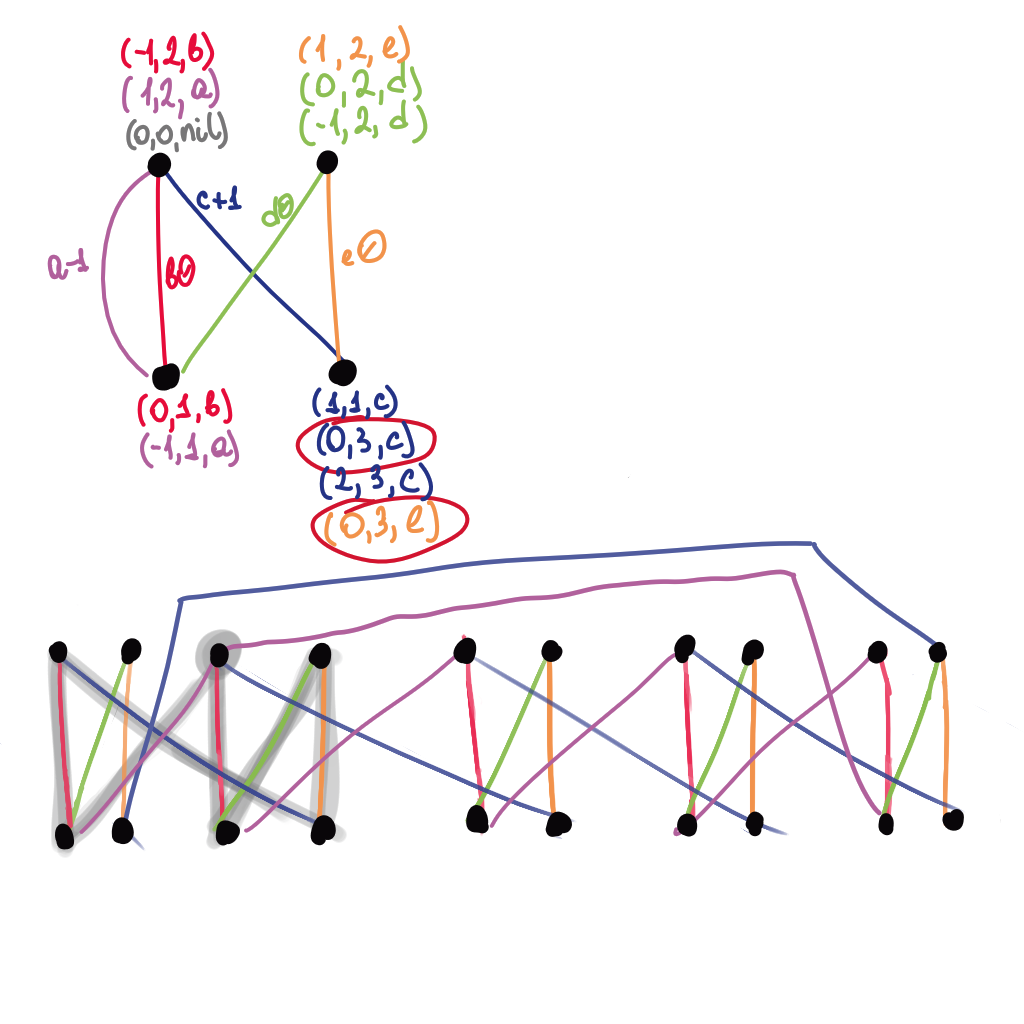
\includegraphics[scale=1.0]{cycle_search.png}
    \caption{ Поиск цикла на метаграфе и соответствующий ему цикл на 5-расширении. }\label{cycle_search}
\end{figure}

\textbf{Замечание.}

Если в алгоритме 1.  учитывать совпадающие характеристики только пометок в текущем поколении, ты будут найдены только циклы состоящие из двух <<крыльев>> одинаковой длины, однако любой цикл на метаграфе представим в таком виде, следовательно будут найдены все циклы.

\textbf{Пример 3.}

% Пример с циклом пробегающим по всему графу, возможно? Чтобы показать, что в таком случае важно именно сравнение по модулю

Рассмотрим ещё один пример работы алгоритма на рис. \ref{cycle_mod_search}. В верхней части рисунка изображён метаграф $G$ с пометками, оставленными алгоритмом поиска циклов. В нижней части рисунка изображено 5-расширение метаграфа $G$, на котором помечен найденный цикл, который проходит по кругу через весь граф.

\begin{figure}[H]
    \centering
    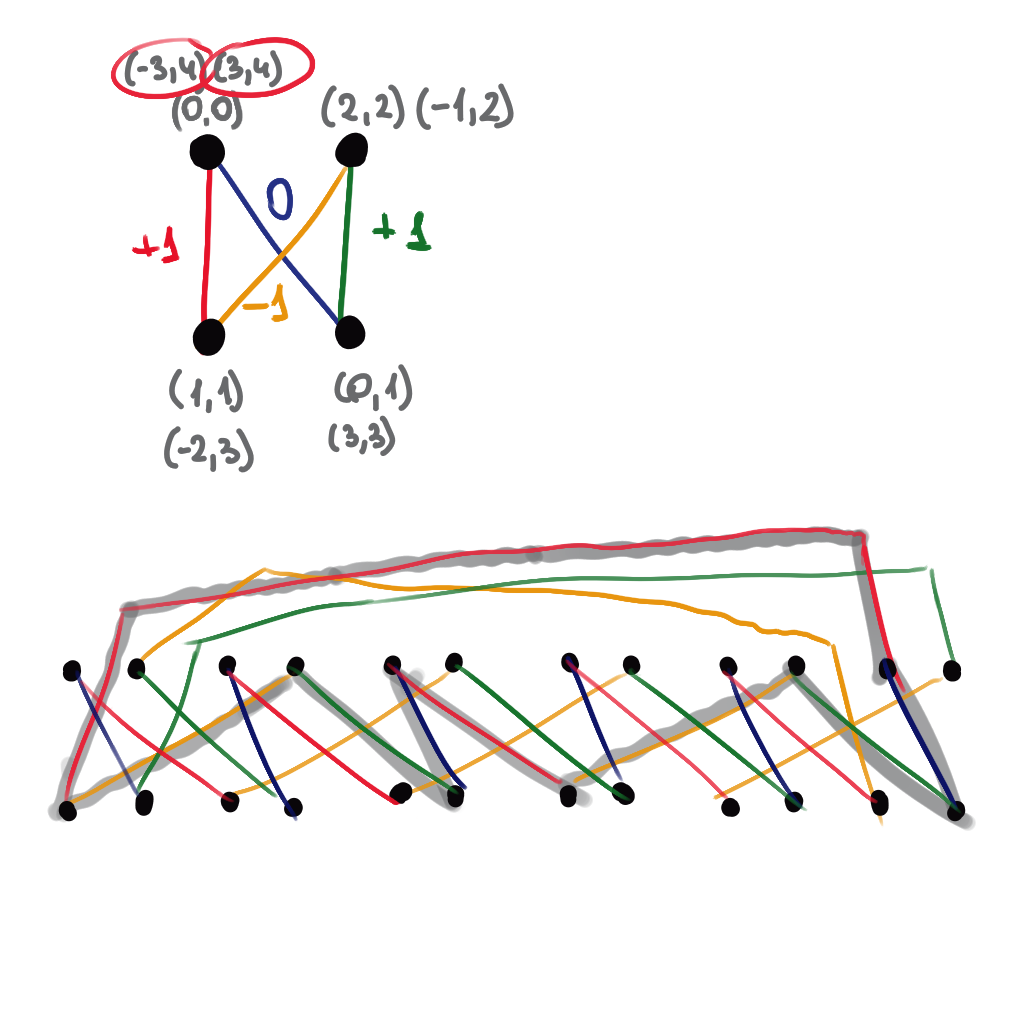
\includegraphics[scale=1.0]{cycle_mod_search.png}
    \caption{ Поиск сквозного цикла на метаграфе и соответствующий ему цикл на 5-расширении. }\label{cycle_mod_search}
\end{figure}


\textbf{Замечание.}

%TODO

О двух видах циклов: которые зависят от $r$ и которые не зависят.

\pagebreak

\section*{Построение графов с заданным обхватом}

Пусть $G = ( V, E, w )$ ~-- метаграф, причём $V = A \cup B$ и $w(e_i) = x_i \forall i = 0..|E|$.

Для каждой пары вершин $a$ и $v$, таких что $a \in A$ и $v \in V$, рассмотрим все неравенства вида $ch(\eta) \neq ch(\mu)$ Где $\eta$ и $\mu$ ~-- различные пути из $a$ в $v$, одинаковой длины не большей некоторого заданного значения $l \in N$.

Систему, содержащую все такие неравенств представим в виде (1).

\begin{equation}
    \centering
    \left\{
        \begin{array}{ll}
            a_{1,1} x_1 + ... + a_{1,e} x_e + b &\neq 0\\
            ...\\
            a_{l,1} x_1 + ... + a_{l,1} x_e + b &\neq 0\\
        \end{array}
    \right.
    \label{eqs:example}
\end{equation}

Пусть $G$ ~-- некоторый метаграф. Тогда справедлива следующая теорема.

\textbf{Теорема 5.}

Для $G$ существует расширение с обхватом большим $2l$  тогда и только тогда, когда система неравенств (1) для графа $G$ совместна.

\textbf{Доказательство.}

Из теоремы 4 следует, что характеристики путей, начинающихся и заканчивающихся в одной вершине равны, тогда и только тогда, когда они образуют цикл. Следовательно, при построении системы (1) ичерпываются все пары путей, которые могли бы образовать цикл. Таким образом существование решения системы (1) эквивалентно существованию расширения с обхватом большим, чем удвоенная длина максимального пути.

\qed

Для построения системы вида \ref{eqs:example} для заданного метаграфа $G$ можно воспользоваться следующим алгоритмом, являющимся модификацией\\ Алгоритма 1.

\textbf{Алгоритм 2.}

Пусть $G = \langle A \cup B, E,w\rangle$ ~-- метаграф причём $w(e_i) = x_i \forall i = 0..|E|$. Для каждой вершины $a \in A:$

\begin{itemize}
    \item Пометим $a$ парой $(0, 0)$.
    \item В цикле по поколениям $g$ от $1$ до $l$:
      \begin{itemize}
      \item Для всех меток $label = (ch, g - 1)$:
        \begin{itemize}
        \item Вершину, которая помечена меткой $label$, обозначим $v$.
        \item Для всех дуг $e: v \in f(e)$:
          \begin{itemize}
          \item $ch' = ch + (-1)^{g} w(e)$
          \item Обозначим $v'$ вершину, такую, что $v' \in f(e), v' \neq v$.
          \item Если $v'$ ещё не была помечена меткой $(ch', g') \forall g'$ ~-- пометим её парой $(ch', g)$.
          \end{itemize}
        \end{itemize}
      \end{itemize}
    \item Возвращаем систему, содержащую все неравенства вида, $ch_1 \neq \ch_2$ для всех пар меток на одной и той же вершине с одним и тем же поколением.
\end{itemize}

$/*$ Пример $*/$

\section*{Решение систем не равенств}

Поиск минимального решения для систем неравенств вида (\ref{eqs:example}), представленных в прошлой главе представляется вычислительно трудной задачей. Она предполагает перебор всех возможных решений с выбором минимального. Однако некоторое решение можно найти, воспользовавшись следующим алгоритмом.

\textbf{Алгоритм 3.}

\begin{enumerate}
    \item $e$ ~-- количество неизвестных в системе неравенств.
    \item Если в системе содержится неравенство вида $0 \neq 0$, то система не имеет решений, алгоритм завершается, сообщая, что решений нет.
    \item Найдём все неравенства вида $a x_e + b \neq 0$. Обозначим множество таких неравенств $I$.
    \item Выберем число $v$ такое, что $v \neq -b/a \forall a x_e + b \in I$, если $I = \varnothing$, то положим $v = 0$. Такое число можно найти, так как неравенств конечное количество. В результате этой замены не возникнет неравенства вида $0 \neq 0$ по условию выбора $v$.
    \item Заменим во всех неравенствах $x_e$ на $v$ и добавим в решение элемент $x_e = v$.
    \item Если $e = 1$ ~-- завершим работу алгоритма.
    \item Положим $e = e - 1$ переменной и вернёмся на шаг 3.
\end{enumerate}

$/*$ Пример $*/$

\textbf{Замечание.}

Результатом работы алгоритма поиска рещшения системы неравенств не обязательно будет минимальное решение.

% Пример

\section*{Оценка работы алгоритма}

Описанный выше алгоритм построения графов с заданным обхватом не обязательно порождает решения с минимальным количеством вершин.

% Пример?

С увеличением требуемого обхвата количество вершин у результирующего графа растёт очень быстро.

Для метаграфа $G = \langle V,E,w \rangle$, количество вершин можно оценить снизу числом $  $ % Надо вспомнить, каким числом мы его оценивали

\textbf{Доказательство.}

% Оценки сверху мы, кажется, никакой не давали

% три пути, смотреть скриншот

% Надо дать оценки r

\end{document}